\documentclass[10pt, a4, serif]{beamer}

%% beamer theme
\usetheme{AnnArbor}
\usecolortheme{crane}

%% Preambles
\usepackage{luatexja}
\usepackage{luatexja-fontspec}
\usepackage{fontspec} %%% fontを変更する:platexにはない
%\usepackage[T1]{fontenc}
\usepackage{lmodern} %%% サンセリフ体の数式記号など
\usepackage{bm} %%% 太字にする
%\usepackage{bxascmac} %%% lualatexでitemboxなどを使う
\usepackage{amsmath} %%% align, gather などのコマンド
\usepackage{amsfonts} %%% たぶんギリシャ文字の太字
\usepackage{color}
\usepackage{graphicx}
%\usepackage[math-style=TeX]{unicode-math}
%\usepackage[dvipdfmx]{hyperref}

\renewcommand\mathfamilydefault{\rmdefault}
%%% FONT platexでコンパイルするときはこのセクションを削除
%\setmainfont{Times New Roman} %%% platexにはない:
%\setmainjfont[BoldFont=Hiragino Kaku Gothic Pro W6]{Hiragino Kaku Gothic Pro W3}
\setmainjfont[BoldFont=FolkPro Bold]{FolkPro Regular}
%\setmainjfont[BoldFont=ShinGoPr5 Bold]{ShinGoPr5 Light}
\setsansfont{Helvetica}
\setsansjfont{Hiragino Maru Gothic Pro W4}
\setmonofont{Consolas}
%%% platexを使う場合ここまで削除

%\def\dif#1{\ \mathrm{d} #1}
%\def\gauss#1{ {\cal N} ( #1 | \mu, \sigma^2 ) }
%\def\infint#1{ \int_{-\infty}^{\infty} #1 \dif{x} }
%\newcommand{\bsf}[1]{\bm{\mathsf{#1}}}
\newcommand{\mbf}[1]{\mathbf{#1}}
\newcommand{\mrm}[1]{\mathrm{#1}}
\newcommand{\trp}[1]{ #1^{\mathrm{T}}}  % 転置
\newcommand{\wt}[1]{\widetilde{#1}}
%\newcommand{\bs}[1]{ {\boldsymbol #1} }

%%% platexを使う場合ここから削除
\newjfontfamily\nfmaporo{NfMotoyaAporo W1 KP}
\newfontfamily\optima{Optima}
\newjfontfamily\mincho{Hiragino Mincho Pro W3}
%%% platexを使う場合ここまで削除

\title{6.4. ガウス過程}
\author{Shunsuke Shigemitsu}
\institute{M2 Bilab@UT}
\date{28, September, 2012}

\begin{document}

% page 1 (title)
\frame{\titlepage}

%% Introduction
% page 2
\frame{
    \frametitle{おさらい}
    カーネル法:
    $y(\mathbf{x}) =
    \mathbf{w}^{\mathrm{T}} {\boldsymbol \phi}(\mathbf{x})$
    のような非線形の写像(基底関数)
    $\boldsymbol \phi$を用いた線形結合を考えるときに、
    カーネル関数
    \begin{align}
    k(\mathbf{x}, \mathbf{x'}) 
    = {\boldsymbol \phi}(\mathbf{x})^{\mathrm{T}}
    {\boldsymbol \phi} (\mathbf{x'})  \tag{6.1}
    \end{align}
    を計算することで、
    $\boldsymbol \phi$による写像を直接計算せずにすむという方法。\\
    (実際の関数は、
    $k(\mathbf{x}, \mathbf{x'}) 
    = \exp( - \| \mathbf{x} - \mathbf{x'} \|^2
    / 2 \sigma^2)$
    みたいな感じ) \vspace{0.2in}

    今回は・・・\\
    これを確率的識別モデルに適用してみる。
}

% page 3
\frame{
    \frametitle{確率過程って?}
    \textbf{確率過程}{\optima(stochastic process)}とは、任意の有限な値集合
        $y(\mathbf{x}_1), \ldots, y(\mathbf{x}_N)$
    に対して、矛盾のない同時分布を与えるもの。\vspace{0.2in}

    → たとえば、時間とともに変化していく確率変数。\\
    確率変数($y(\mathbf{x})$とか)がたくさんあって、それを全部まとめたものが
    確率過程。その中から適当に$N$個を取り出したときの確率分布を考える。\\
    実生活で目にする(?)ものでいうと、ブラウン運動などがある。\vspace{0.2in}

    \textbf{ガウス過程}{\optima(Gaussian process)}は、確率過程の中でも
    たくさんの$y(\mathbf{x})$の同時分布$p(y(\mathbf{x}_1), \ldots, y(\mathbf{x}_N))$
    がガウス分布に従うようなもののこと。
}


%% 6.4.1 Linear Regression again

% page 4
\frame{
    \frametitle{6.4.1 線形回帰モデル再び}
    3章でやった線形回帰モデルを用いる。

    \begin{align}
        y(\mathbf{x}, \mathbf{w}) 
        = \mathbf{w}^{\mathrm{T}} {\boldsymbol \phi} (\mathbf{x}) 
        &\ 
        &\text{\nfmaporo ...(6.49) モデルはこんな感じ} \notag \\
        \mathbf{w} &\  &\text{\nfmaporo ... パラメータベクトル($M$次元)} \notag \\
        {\boldsymbol \phi}  &\ 
        &\text{\nfmaporo ... 非線形な写像、基底関数。$M$個ある} \notag \\
        \mathbf{x} &\ &\text{\nfmaporo ... 入力値} \notag
    \end{align}

    流れ:
    \begin{itemize}
    \item $\mathbf{w}$の事前分布($p(\mathbf{w})$)を決める
    \item 関数$y(\mathbf{x}, \mathbf{w})$に対する事前分布も決まる。
    \item 訓練データの集合$\mathbf{x}_1, \ldots, \mathbf{x}_N$が与えられると、
    今度は$\mathbf{w}$の事後分布$p(\mathbf{w}|\mathbf{x}_1, \ldots, \mathbf{x}_N)$
    が求まる。
    \item そこから最終的な目的である新しい入力ベクトル$\mathbf{x}$に対する
    予測分布$p(t|\mathbf{x})$ が求まる。(→6.4.2節)
    \end{itemize}
}

% page 5
\frame{
    \frametitle{線形回帰ふたたび(2)}
    まずは、パラメータ$\mathbf{w}$の事前分布を決める(どんな分布なのか
    よくわからないので、適当に決める)。
    \begin{gather}
    p(\mathbf{w}) 
    = {\cal N} (\mathbf{w} | \mathbf{0}, \alpha^{-1} \mathbf{I}).
    \tag{6.50}
    \end{gather}

    このとき、$\alpha$は超パラメータで、分布の精度を表す(大きければ大きいほど
    ばらつきが少ない)。

    特定の$\mathbf{w}$が決まると、$\mathbf{x}$についての特定の関数$y(\mathbf{x})$
    が決まる。ここで、回帰を行うには、訓練データ点の集合
    $\mathbf{x}_1, \ldots, \mathbf{x}_N$における関数(の集合)を評価したい。
    その関数の値の集合を、要素
    \begin{gather}
    y_n = y(\mathbf{x}_n)\ \ (n = 1, \ldots, N) \notag
    \end{gather}
    を持つようなベクトル$\bm{\mathsf{y}}$として表す。(6.49)式を$\bm{\mathsf{y}}$
    を用いてまとめると、
    \begin{gather}
    \bm{\mathsf{y}} = {\boldsymbol \Phi} \mathbf{w} \tag{6.51}
    \end{gather}
    となる。ただし、$\boldsymbol \Phi$は要素$\phi_{nk} = \phi_k (\mathbf{x}_n)$
    をもつような計画行列。
}

% page 6
\frame{
    \frametitle{線形回帰再び(3)}
    $\bm{\mathsf{y}}$はガウス分布に従う$\mathbf{w}$の線形結合なので、
    $\bm{\mathsf{y}}$もガウス分布に従う。ということは、平均と共分散がわかれば、
    $\bm{\mathsf{y}}$がどんなものなのかがわかる。
    (6.50)式($p(\mathbf{w}) 
    = {\cal N} (\mathbf{w} | \mathbf{0}, \alpha^{-1} \mathbf{I})$)より、

    \begin{align}
    \mathbb{E}[\bm{\mathsf{y}}]
        &= {\boldsymbol \Phi} \mathbb{E}[\mathbf{w}] = \mathbf{0}
    \tag{6.52} \\
    \mathrm{cov}[\bm{\mathsf{y}}]
        &= \mathbb{E}[\bm{\mathsf{yy}}^{\mathrm{T}}]
        = {\boldsymbol \Phi} \mathbb{E} [\mathbf{ww}^{\mathrm{T}}]
          {\boldsymbol \Phi}^{\mathrm{T}}
        = \frac{1}{\alpha} {\boldsymbol \Phi \boldsymbol \Phi}^{\mathrm{T}}
        = \mathbf{K}
    \tag{6.53}
    \end{align}
    となる。なお、$\mathbf{K}$は、
    \begin{gather}
    K_{nm} = k(\mathbf{x}_n, \mathbf{x}_m)
        = \frac{1}{\alpha} {\boldsymbol \phi} (\mathbf{x}_n)^\mathrm{T}
          {\boldsymbol \phi} (\mathbf{x}_m)
    \tag{6.54}
    \end{gather}
    を要素に持つグラム行列である。
}

% page 7
\frame{
    \frametitle{なにがすごいの?}
    $N$個の変数の同時分布が、平均と共分散だけで表せてしまうというところが
    すごい。

    ちなみに、$y(\mathbf{x})$の平均は、事前知識がない場合対称性から0とすることが多い。
    これは、($y(\mathbf{x})$を決める)パラメータの事前分布
    $p(\mathbf{w}|\alpha)$の平均を0にするのと同じことである。\vspace{0.2in}
    
    このとき、ガウス過程は、カーネル関数
    \begin{gather}
    \mathbb{E}[y(\mathbf{x}_n) y(\mathbf{x}_m)]
        = k(\mathbf{x}_n, \mathbf{x}_m)
    \tag{6.55}
    \end{gather}
    で与えられる共分散によって定まる。\\
    (ガウス過程は$y(\mathbf{x})$の寄せ集めで、
     実際の$\mathbf{w}$はいろんなものがあり得る)
}

% page 9
\frame{
    \frametitle{図解}
    カーネル関数$k$は、基底関数$\boldsymbol \phi$を決めることで求めることも
    できるが、実際は直接定義することのほうが多い(たぶん)。下図は、
    異なる2つのカーネル関数で定まるガウス過程からサンプルされた関数を示す。

  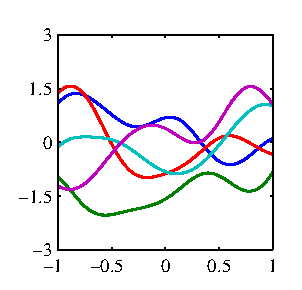
\includegraphics[clip, width=3cm]{charts/Figure6_4a.eps}
  \hspace{1cm}
  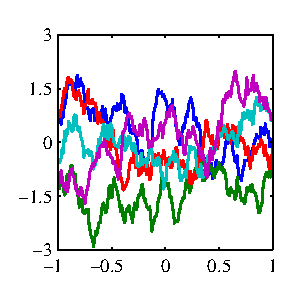
\includegraphics[clip, width=3cm]{charts/Figure6_4b.eps}

  左:
  $k(\mathbf{x}, \mathbf{x'}) = 
  \exp( - \|\mathbf{x} - \mathbf{x'}\|^2 / 2\sigma^2)
  $ {\optima (6.23)}

  右:
  $k(x, x') = \exp( - \theta |x - x'|)$ {\optima (6.56)} 

  \vspace{0.6cm}
  {\optima(6.56)}は、もともとは\textbf{オルンシュタインーウーレンベック過程}
  {\optima(Ornstein-Uhlenbeck process)}というブラウン運動を記述するために
  作られたモデル。

  %  \begin{figure}[htbp]
  %\begin{center}
  %  \begin{tabular}{c}

  %    % 1
  %    \begin{minipage}{0.33\hsize}
  %      \begin{center}
  %        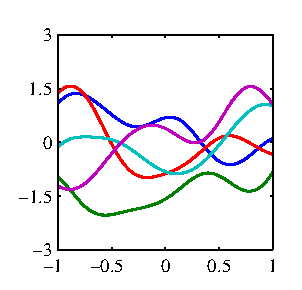
\includegraphics[clip, width=4.5cm]{charts/Figure6_4a.eps}
  %        \hspace{1.6cm} [1]
  %        $k(\mathbf{x}, \mathbf{x'}) = 
  %        \exp( - \|\mathbf{x} - \mathbf{x'}\|^2 / 2\sigma^2)
  %        $ {\optima (6.23)}
  %      \end{center}
  %    \end{minipage}

  %    % 2
  %    \begin{minipage}{0.33\hsize}
  %      \begin{center}
  %        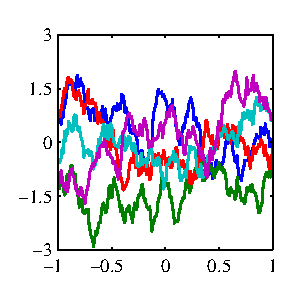
\includegraphics[clip, width=4.5cm]{charts/Figure6_4b.eps}
  %        \hspace{1.6cm} [2]
  %        $k(x, x') = 
  %        \exp( - \theta |x - x'|)
  %        $ {\optima (6.56)}
  %      \end{center}
  %    \end{minipage}

  %\end{tabular}
  %\end{center}
  %\end{figure}
}

% page 8
\frame{
    \frametitle{より一般的には...}
    ガウス過程とは、$y(\mathbf{x})$がガウス分布に従うような確率過程の
    ことである(つまり、関数の形は必ずしも
    $y(\mathbf{x})=\mathbf{w}^\mathrm{T} {\boldsymbol \phi}(\mathbf{x})$
    でなくてもよい)。\vspace{0.2in}

    入力ベクトルが2次元のときは、特別に\textbf{ガウス確率場}
    {\optima(Gaussian random field)}と呼ばれる。
}

% page 9
\frame{
    \frametitle{6.4.1 まとめ}
    \begin{itemize}
    \item ガウス過程とは、関数の値の集合$\bm{\mathsf{y}}$の同時確率が、
    ガウス分布に従うような確率過程(確率変数の寄せ集め)のこと。
    \item 線形回帰も、パラメータ$\mathbf{w}$がガウス分布に従うとすると、
    各データ点$\mathbf{x}_1, \ldots, \mathbf{x}_N$が与えられた
    時の関数の値$\bm{\mathsf{y}}$もガウス分布に従うので、ガウス過程である。
    \item $y(\mathbf{x})$を
        $y(\mathbf{x}) = \mathbf{w}^\mathrm{T} {\boldsymbol \phi} (\mathbf{x})$
    とすると、
    \begin{align}
    \mathbb{E}[\bm{\mathsf{y}}]
        &= {\boldsymbol \Phi} \mathbb{E}[\mathbf{w}] = \mathbf{0}
    \tag{6.52} \\
    \mathrm{cov}[\bm{\mathsf{y}}]
        &= \mathbb{E}[\bm{\mathsf{yy}}^{\mathrm{T}}]
        = \frac{1}{\alpha} {\boldsymbol \Phi \Phi}^{\mathrm{T}}
        = \mathbf{K} \tag{6.53}% \\
    %\mathbb{E}[y(\mathbf{x}_n) y(\mathbf{x}_m)]
    %    &= k(\mathbf{x}_n, \mathbf{x}_m)
    %\tag{6.55}
    \end{align}
    で表されるような確率過程となる。
    \item カーネル関数をどんなものにするかによって、サンプリングされる関数の
        形も変わってくる。
    \end{itemize}
}


%% 6.4.2 Regression by Gaussian process
% page 10
\frame{
    \frametitle{6.4.2 ガウス過程による回帰}
    出てくる変数:
    \begin{itemize}
        \item $t_n$ :観測変数。$y_n = y(\mathbf{x}_n)$として、
            \begin{gather}
                t_n = y_n + \epsilon_n \tag{6.57}
            \end{gather}
            で定義される。
            まとめて$\bm{\mathsf{t}} = (t_1, \ldots, t_N)^\mathrm{T}$.
        \item $\epsilon_n$ :ノイズ。それぞれの観測値に対して独立に決まる。
           $\beta$をノイズの精度を表す超パラメータとして、
           \begin{gather}
                p(t_n|y_n) = {\cal N} (t_n | y_n, \beta^{-1}) \tag{6.58}
            \end{gather}
            となる。
    \end{itemize}
            
}

% page 11
\frame{
    \frametitle{N個の訓練集合をまとめて書く}
    ノイズは各データ点($y(\mathbf{x}) = $真の値)に対してランダムに決まるので、
    {\optima (6.58)}式をまとめて書くと、
    \begin{gather}
    p(\bm{\mathsf{t}}|\bm{\mathsf{y}})
        = {\cal N} (\bm{\mathsf{t}} | \bm{\mathsf{y}}, 
                \beta^{-1} \mathbf{I}_N).
    \tag{6.59}
    \end{gather}
    となる。ただし、$\mathbf{I}_N$は$N \times N$の単位行列。

    ガウス過程の定義($\mathbb{E}[\bm{\mathsf{y}}] = \mathbf{0}$, 
            $\mathrm{cov}[\bm{\mathsf{y}}] = \mathbf{K}$)より、
    周辺分布$p(\bm{\mathsf{y}})$は、
    \begin{gather}
    p(\bm{\mathsf{y}}) = {\cal N} (\bm{\mathsf{y}} | \mathbf{0}, \mathbf{K}).
        \tag{6.60}
    \end{gather}
    である。

    $\mathbf{K}$を決めるカーネル関数は、二つの点$\mathbf{x}_n$と$\mathbf{x}_m$が
    似ているほど$y(\mathbf{x}_n)$と$y(\mathbf{x}_m)$の相関が高いようなもの
    が選ばれる(たとえばガウスカーネル)。
}

% page 12
\frame{
    \frametitle{データ点のサンプリング}
    \begin{figure}
        \begin{center}
            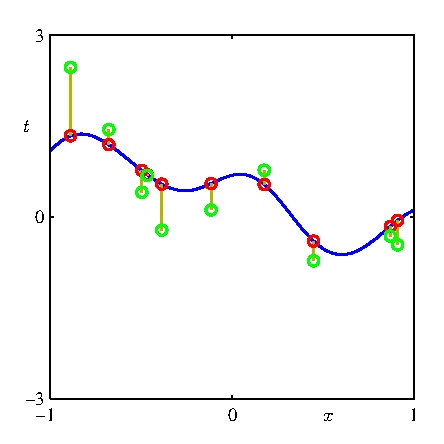
\includegraphics[width=5cm]{charts/Figure6_6.eps}
            \label{6.6}
            \caption{
                \textcolor{blue}{実線}はガウス過程からサンプリングした関数、
                \textcolor{red}{赤い点}
                は入力集合${x_n}$に対応する値$y_n$を表す。\textcolor{green}{緑の丸}
                は、${y_n}$にそれぞれ独立にガウスノイズを加えた点${t_n}$
                を示している。
            }
        \end{center}
    \end{figure}
}

% page 13
\frame{
    \frametitle{観測値の周辺分布}
    $p(\bm{\mathsf{t}} | \bm{\mathsf{y}})$と$p(\bm{\mathsf{y}})$がわかったので、
    次は周辺分布$p(\bm{\mathsf{t}})$を求めたい。すなわち、{\optima (2.115)}式(
    $x$)を用いて、

    \begin{gather}
        p(\bm{\mathsf{t}}) = 
        \int p(\bm{\mathsf{t}} | \bm{\mathsf{y}}) 
            p(\bm{\mathsf{y}}) \d \bm{\mathsf{y}}
        = {\cal N} (\bm{\mathsf{t}} | \mathbf{0}, \mathbf{C}).
        \tag{6.61}
    \end{gather}

    と求まる。共分散行列$\mathbf{C}$の各要素は、
    \begin{gather}
        C(\mathbf{x}_n, \mathbf{x}_m)
        = k(\mathbf{x}_n, \mathbf{x}_m) + \beta^{-1} \gamma_{nm}
        \tag{6.62}
    \end{gather}
    である。$y(\mathbf{x})$と$\epsilon$が互いに独立であるため、共分散もこの二つを
    足し合わせるだけで良い。
}

% page 14
\frame{
    \frametitle{新しい入力を予測する}
    $p(\bm{\mathsf{t}} | \bm{\mathsf{y}})$と$p(\bm{\mathsf{y}})$、
    $p(\bm{\mathsf{y}})$が求まったので、新しい入力ベクトル$\mathbf{x}_{N+1}$
    に対する目標変数$t_{N+1}$を予測したい。そのためには、予測分布
    $p(t_{N+1}|\bm{\mathsf{t}}_N)$を求めなければならない(
    $\bm{\mathsf{t}}_N = (t_1, \ldots, t_N)^{\mathrm{T}}$)。
    
    このとき、
    $p(t_{N+1}|\bm{\mathsf{t}}_N)$は$\bm{\mathsf{t}}_N$だけでなく
    $\mathbf{x}_1, \ldots, \mathbf{x}_N, \mathbf{x}_{N+1}$にも依存しているが、
    簡単のためにそこは省略。\vspace{0.2in}

    {\optima(6.61)}より、$t_1, \ldots, t_{N+1}$の同時分布は、
    \begin{gather}
        p(\bm{\mathsf{t}}_{N+1})
        = {\cal N} (
            \bm{\mathsf{t}}_{N+1} |
            \mathbf{0}, \mathbf{C}_{N+1}
            ).
        \tag{6.64}
    \end{gather}

    このとき、$\mathbf{C}_{N+1}$は、$(N+1) \times (N+1)$の共分散行列で、
    各要素は前頁の{\optima(6.62)}式で与えられる。この式から予測分布を
    求めることができる。
}

% page 15
\frame{
    \frametitle{回帰で求める平均と分散}
    {\optima(6.64)}式の$\mathbf{C}_{N+1}$を分割して、
    \begin{gather}
        \mathbf{C}_{N+1} = 
        \begin{pmatrix}
            \mathbf{C}_N & \mathbf{k} \\
            \mathbf{k}^{\mathrm{T}} & c
        \end{pmatrix}
        \tag{6.65}
    \end{gather}
    とする。$\mathbf{k}$は、要素
    $k(\mathbf{x}_n, \mathbf{x}_{N+1} (n = 1, \ldots, N)$を持つ
    ベクトルであり、$c = k(\mathbf{x}_{N+1}, \mathbf{x}_{N+1}) + \beta^{-1}$
    とする。\vspace{0.2in}

    いろいろ計算すると、$p(t_{N+1} | \bm{\mathsf{t}})$は、以下のような平均と
    共分散を持つガウス分布であることがわかる。
    \begin{align}
        m(\mathbf{x}_{N+1}) 
            &= \mathbf{k}^\mathrm{T} \mathbf{C}_{N}^{-1} \bm{\mathsf{t}}
            \tag{6.66} \\
        \sigma^2 (\mathbf{x}_{N+1}) 
            &= c - \mathbf{k}^\mathrm{T} \mathbf{C}_N^{-1} \mathbf{k}
            \tag{6.67}
    \end{align}
}

% page 16
\frame{
    \frametitle{ガウス過程による回帰:例}

    \begin{figure}
        \begin{center}
            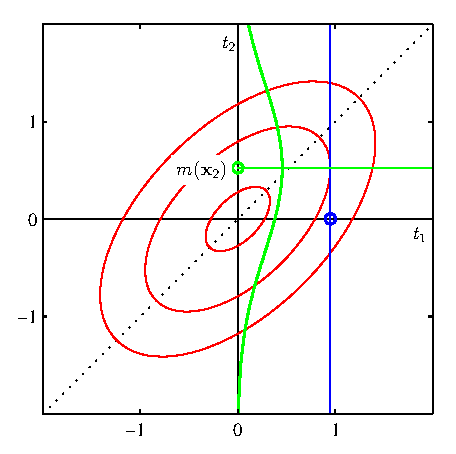
\includegraphics[width=5cm]{charts/Figure6_7.eps}
            \label{6.7}
            \caption{
                訓練データとテストデータが1つずつの場合のガウス過程
                による回帰のしくみ。\textcolor{red}{赤色の楕円}が、
                同時分布$p(t_1, t_2)$の 等高線を示している。$t_1$は
                訓練データ(\textcolor{blue}{青い点})。
                \textcolor{green}{緑色の線}は$p(t_2|t_1)$。
                楕円を青いところで切るとこんな感じになる。
            }
        \end{center}
    \end{figure}
}

% page 17
\frame{
    \frametitle{ガウス過程の適用例}
    \begin{figure}
        \begin{center}
            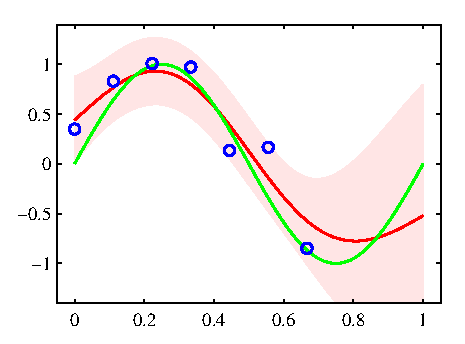
\includegraphics[width=4cm]{charts/Figure6_8.eps}
            \caption{
                \textcolor{red}{赤い線}は正弦関数を表している。
                \textcolor{blue}{青い点}はそこからガウス分布に従う
                ノイズを加えてサンプリングされたデータ点。
                \textcolor{green}{緑色の実線}がガウス過程による平均、
                \textcolor{red}{ピンク色の領域}がガウス過程による分散
                (標準偏差の2倍)を表している。データが疎な部分(右端付近)
                では不確かさ(分散)が大きくなっているのがわかる。
            }
        \end{center}
    \end{figure}
}

% page 18
\frame{
    \frametitle{よく使われるカーネル}
    ガウス過程回帰に使われるカーネル関数として、以下のようなものがある。

    4つの超パラメータ($\theta_0, \theta_1, \theta_2, \theta_3$)をもつ。
    \begin{gather}
        k(\mathbf{x}_n, \mathbf{x}_m)
        = \theta_0 \exp \left\{
            - \frac{\theta_1}{2} \| \mathbf{x}_n - \mathbf{x}_m \|^2
        \right\}
        + \theta_2
        + \theta_3 \mathbf{x}_n^{\mathrm{T}} \mathbf{x}_m.
        \tag{6.63}
    \end{gather}

    \begin{figure}
        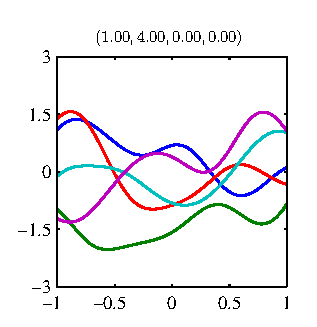
\includegraphics[width=2cm]{charts/Figure6_5a.eps}
        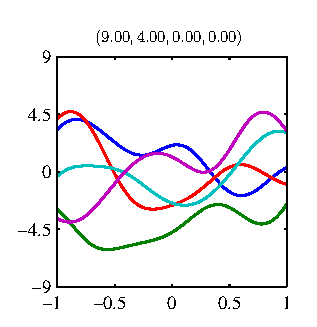
\includegraphics[width=2cm]{charts/Figure6_5b.eps}
        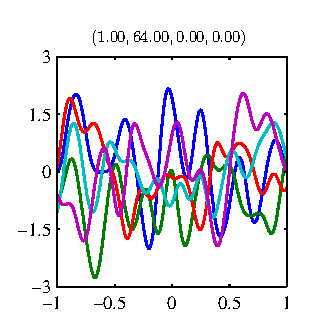
\includegraphics[width=2cm]{charts/Figure6_5c.eps}

        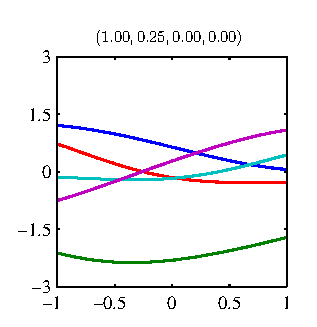
\includegraphics[width=2cm]{charts/Figure6_5d.eps}
        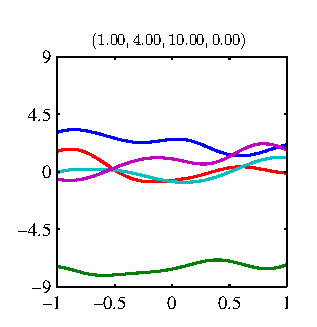
\includegraphics[width=2cm]{charts/Figure6_5e.eps}
        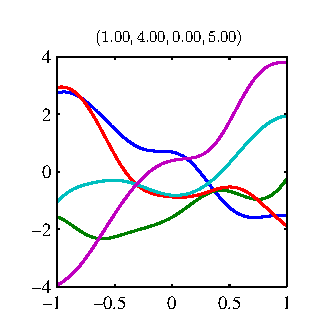
\includegraphics[width=2cm]{charts/Figure6_5f.eps}
    \end{figure}
}

% page 19
\frame{
    \frametitle{制約など}
    カーネル関数は何でも良いが、{\optima(6.62)}で与えられる共分散行列が
    正定値でなければならない。\vspace{0.2in}

    また、予測分布の平均{\optima(6.66)}は、$\mathbf{x}_{N+1}$の関数として
    \begin{gather}
        m(\mathbf{x}_{N+1}) = \sum_{n=1}^N a_n k(\mathbf{x}_n, \mathbf{x}_{N+1})
        \tag{6.68}
    \end{gather}
    と表すことができる。ただし、$a_n$は$\mathbf{C}_N^{-1} \bm{\mathsf{t}}$の
    $n$番目の要素。この式を用いると、$\mathbf{K}$($N \times N$次元)の代わりに
    $M$個の基底関数で表すことができ、$M \times M$の行列の逆行列を求めればすむ。
    
    このため、データ数$N$に比べてモデル数$M$が少ないような場合は、計算量を減らす
    ことができる。ただし、カーネル関数の中には無限個の基底関数でしか表せないものが
    あり、そうしたものにはこの方法は使えない。
}

% page 20
\frame{
    \frametitle{6.4.2 まとめ}
    \begin{itemize}
        \item ノイズ$\epsilon_n$を加えた観測値$\bm{\mathsf{t}}$
            から、新たなデータに対する予測分布$p(t_{N+1}|\bm{\mathsf{t}})$
            を求めることができた。
        \item 予測分布は、
            \begin{align}
        m(\mathbf{x}_{N+1}) 
            &= \mathbf{k}^\mathrm{T} \mathbf{C}_{N}^{-1} \bm{\mathsf{t}}
            \tag{6.66} \\
        \sigma^2 (\mathbf{x}_{N+1}) 
            &= c - \mathbf{k}^\mathrm{T} \mathbf{C}_N^{-1} \mathbf{k}
            \tag{6.67}
    \end{align}
    という平均と共分散を持つガウス分布になる。
\item $N \times N$の共分散行列の逆行列$\mathbf{C}_N^{-1}$を求めなければならないので、
    計算時間は$O(N^3)$となってしまう。基底関数を用いて$\mathbf{S}_N$の逆行列を求めれば
    (カーネルトリックは使えないが)計算量は$O(M^3)$になる。

    \end{itemize}
}


%% 6.4.3 Learning hyper parameters
% page 21
\frame{
    \frametitle{6.4.3 超パラメータの学習}
    ガウス過程による予測は、共分散を決める際の超パラメータに依存している。
    実際の応用では、あらかじめ超パラメータを決めておくよりも、これを学習
    させることが多い。

    超パラメータの学習は、尤度関数$p(\bm{\mathsf{t}} | {\boldsymbol \theta})$
    に基づいて行われることが多い。最も単純なアプローチは、対数尤度関数
    $\ln p(\bm{\mathsf{t}} | {\boldsymbol \theta})$を最大化するような
    $\boldsymbol \theta$を求めるという方法である。\vspace{0.2in}

    ガウス過程における対数尤度関数は、
    \begin{gather}
    \ln p(\bm{\mathsf{t}} | {\boldsymbol \theta}) 
        = - \frac{1}{2} \ln | \mathbf{C}_N |
        - \frac{1}{2} \bm{\mathsf{t}}^\mathrm{T} \mathbf{C}_N^{-1} \bm{\mathsf{t}}
        - \frac{N}{2} \ln (2 \pi)
    \tag{6.69}
    \end{gather}
    で与えられる。
}

% page 22
\frame{
    \frametitle{対数尤度関数の最大化}

    先ほどの続きで、パラメータベクトル$\boldsymbol \theta$の勾配も求める。
    \begin{align}
    \frac{\partial}{\partial x} (\mathbf{A}^{-1})
       &= - \mathbf{A}^{-1} 
            \frac{\partial \mathbf{A}}{\partial x}
            \mathbf{A}^{-1}
    \tag{C.21} \\
    \frac{\partial}{\partial x} \ln |\mathbf{A}|
       &= \mathrm{Tr} \left(
               \mathbf{A}^{-1} \frac{\partial \mathbf{A}}{\partial x}
               \right)
       \tag{C.22}
    \end{align}
    を用いて(付録C参照)、
    \begin{gather}
    \frac{\partial}{\partial \theta_i} \ln p(\bm{\mathsf{t}} | {\boldsymbol \theta})
        = - \frac{1}{2} \mathrm{Tr} \left(
                \mathbf{C}_N^{-1} \frac{\partial \mathbf{C}_N}{\partial \theta_i}
                \right)
        + \frac{1}{2} \bm{\mathsf{t}}^\mathrm{T} \mathbf{C}_N^{-1}
          \frac{\partial \mathbf{C}_N}{\partial \theta_i}
          \mathbf{C}_N^{-1} \bm{\mathsf{t}}
    \tag{6.70}
    \end{gather}
    である。ただし、$\ln p(\bm{\mathsf{t}} | {\boldsymbol \theta})$は非凸関数なので
    極大点は複数あり得る。
}

\frame{
    \frametitle{6.4.3 まとめ}
    \begin{itemize}
    \item ガウス過程に現れる超パラメータの学習は、対数尤度の最大化という
        一般的な手法が用いられることが多い。
    \item ただし対数尤度関数はカーネル関数のせいで非線形なことが多いので、
        そうした場合は超パラメータの勾配も求める必要がある。
    \item ベイズ的な手法を用いて予測することもあるが、その際は近似を用いなければ
        ならない($p({\boldsymbol \theta})$や$p(\bm{\mathsf{t}}|{\boldsymbol \theta})$
        を厳密に周辺化することができない)。
    \end{itemize}
}

\end{document}
